\begin{frame}
	\frametitle{O neurônio \textit{Leaky Integrate-and-Fire} (LIF)}
	\only<1>{
		\framesubtitle{O modelo RC}
		\begin{columns}
			\column{.60\linewidth}
			\begin{itemize}
				\item O LIF se comporta como um circuito Resistor-Capacitor (RC).
				\item $R$: resistência de vazamento; $C$: capacitância; $V_{mem}$: potencial acumulado; $\vartheta$: interruptor que descarrega o capacitor (dispara um pulso) ao atingir o limiar.
				\item Governado por \cite{eshraghian2023training}:
				
				
				 $\tau\frac{dV_{mem}}{dt} = R\,I_{in}(t) - V_{mem}(t)$, com $\tau = R\cdot C$ .
			\end{itemize}
			\column{.40\linewidth}
			\begin{center}
				\includegraphics[width=.85\linewidth]{../../00-thesis/monography/images/rcmodel}\par
				{\tiny Fonte: \cite{eshraghian2023training}}
			\end{center}
		\end{columns}
	}
	\only<2>{
		\framesubtitle{Exemplo numérico: decaimento sem entrada}
		\par Sem corrente ($I_{in}=0$), a equação do slide anterior vira $\tau\,dV_{mem}/dt = -V_{mem}$. Separando as variáveis e integrando os dois lados:
		\begin{equation*}
			\begin{aligned}
				\frac{dV_{mem}}{V_{mem}} = -\frac{dt}{\tau}
				\ & \Rightarrow\
				\int \frac{dV_{mem}}{V_{mem}} = \int -\frac{dt}{\tau}
				\ \Rightarrow\
				\ln V_{mem} = -\frac{t}{\tau} + k \\
				& \Rightarrow\ V_{mem}(t) = e^{k}\cdot e^{-t/\tau}
				\ \Rightarrow\
				V_{mem}(t) = V_{mem}(0)\cdot e^{-t/\tau}
			\end{aligned}
		\end{equation*}
		\par {\small (pois em $t=0$: $e^{k}=V_{mem}(0)$)}
		\par Com $R=5\,\Omega$, $C=1\,F$ (logo $\tau = R\cdot C = 5$) e potencial inicial $V_{mem}(0)=1$:
		\begin{equation*}
			V_{mem}(1) = 1 \cdot e^{-1/5} \approx 0{,}8187
		\end{equation*}
		\par O potencial \textbf{vaza} exponencialmente na ausência de estímulo --- daí o nome \textit{leaky}. Quando um estímulo chega, o potencial sobe (mesma matemática, sinal oposto) até cruzar um limiar $V_{th}$, disparando um pulso e reiniciando.
	}
	\only<3>{
		\framesubtitle{Comportamento completo simulado}
		\begin{center}
			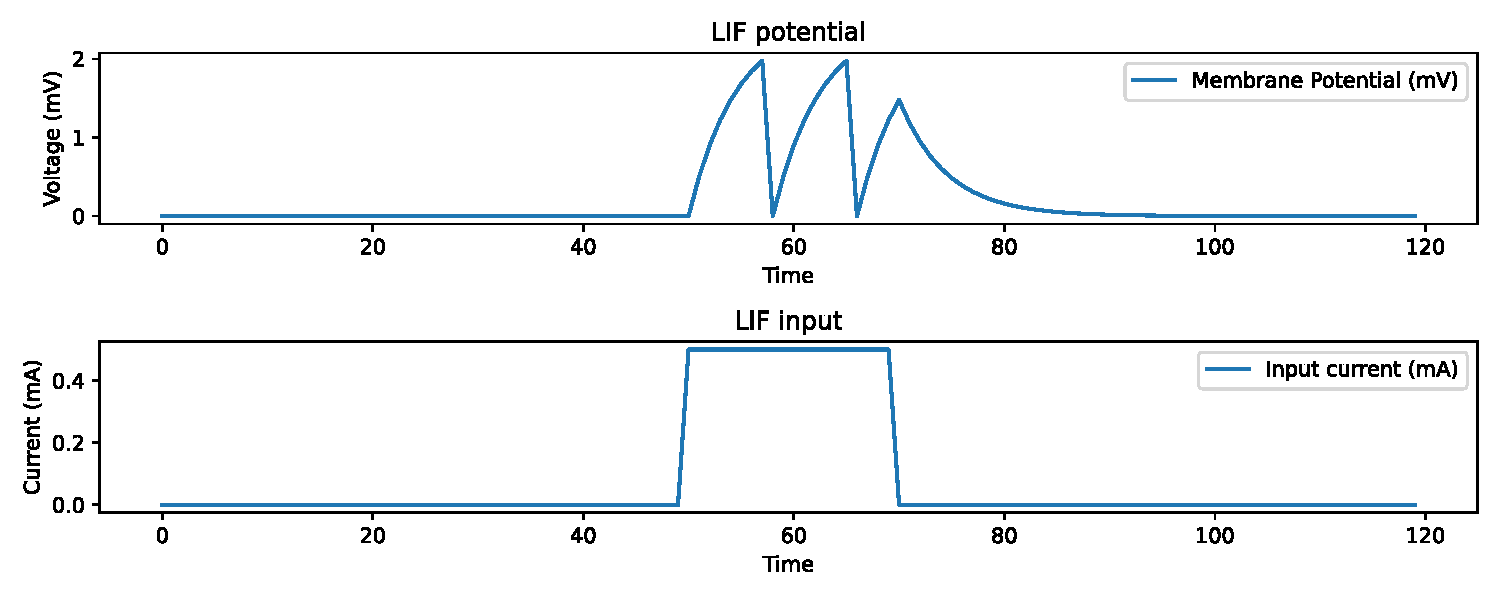
\includegraphics[width=1\linewidth]{../../00-thesis/monography/images/membranePotentialFull}\par
			{\tiny Corrente de 0,5 mA injetada entre os passos 51 e 70. Fonte: elaborado pelo autor.}
		\end{center}
	}
\end{frame}
